\chapter{Materials and methods}
\label{materias_methods}

\section{Device}
\label{mm_device}

Based on some previous works (see, for instance, Sokolov et al.~\cite{Sokolov2007}), and taking into account the microscope dimensions, we designed the baseline of the device as shown in Fig. \ref{device_baseline}. It consists of two quadrilateral frames, the outer being fixed, the inner with a sliding degree of freedom in the Y axis. Each of the frames has two nylon threads attached to it in a way that the relative motion of the frames allows the control of the area enclosed by the threads.

\begin{figure}[H]
	\centering
	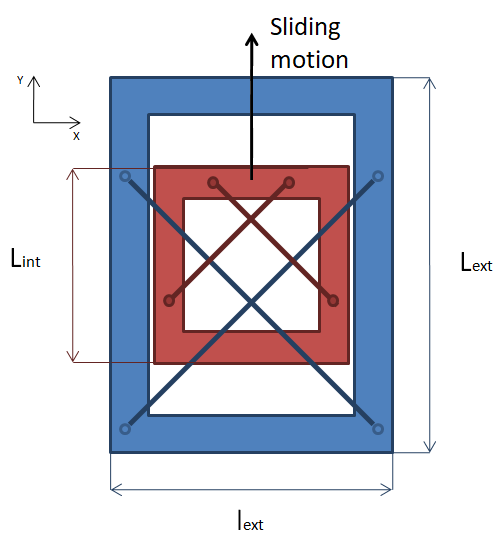
\includegraphics[width=0.4\textwidth]{archivos/baseline_device.png}
	\caption{Diagram of the baseline device}
	\label{device_baseline}
\end{figure}

The device had to accomplish two main objectives: 

\begin{itemize}
	\item to help prevent the influence of the boundary contitions, the minimum size of the stretched central square should have approximately a $6 \; \textrm{mm}$ long side; 
	\item and the size of the central square had to be small enough to hold a $2 \; \mu \textrm{L}$ spherical droplet when the device was shrunk. 
\end{itemize}

Since, at 40x magnification, we will examine $435 \; \mu \textrm{m}$ side squares, the maximum size intends to minimize the effects of the boundary conditions. The Stokes' paradox establishes that perturbations can be quite long ranged, but by looking at the center of the film we expect to be similar enough to the periodic boundary conditions considered in the simulations.

However, the second of this requirements was harder to foresee, and, knowing that the threads were flexible, somehow less important. This led us to the following measures:

\begin{equation}
	L_{ext} = 40 \; \textrm{mm}; \quad l_{ext} = 28 \; \textrm{mm}; \quad L_{int} = 20 \; \textrm{mm}; \quad t = 3.8 \; \textrm{mm}
\end{equation}

where $t$ represents the thickness of both frames.

For the threads we used a $50 \; \mu \textrm{m}$ diameter fishing line (see Fig. \ref{fishing_line}) that we glued to the frames . The frames were laser-cut from a $6 \; \textrm{mm}$ thick sheet.

\begin{figure}[H]
	\centering
	\includegraphics[width=0.3\textwidth]{archivos/fishing_line.jpg}
	\caption{Asso® micron 3 fishing line (D $50 \; \mu \textrm{m}$)}
	\label{fishing_line}
\end{figure}

To hold both frames at the same level, a thinner plastic sheet was glued to the bottom of the outer one.

The relative motion is achieved through the use of a $3 \; \textrm{mm}$ diameter screw. The external frame is drilled and threaded, whereas the internal one is only drilled. Finally, to prevent the screw from sliding back and forth relatively to the inner frame, we place two blocks on both sides of the drill hole.   

\begin{figure}[H]
	\centering
	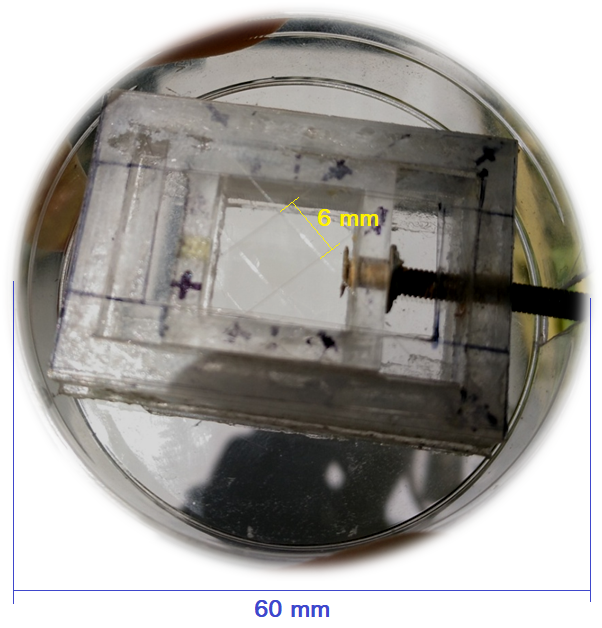
\includegraphics[width=0.4\textwidth]{archivos/device.png}
	\caption{Picture of the device}
	\label{device}
\end{figure}

Previous experiences, such as those of Guasto et al.~\cite{Guasto}, revealed that, at about $25^\textrm{o}\textrm{C}$, the evaporation was too intense for the film to hold long enough to obtain a sufficient number of images at the sought-after thickness. Their solution (and ours) to this problem consisted in enclosing the device in a small box. For this purpose we chose a petri dish (Fig. \ref{petri_dish}). We also placed a humid cotton inside the chamber to increase the saturation levels of the air within it.

\begin{figure}[H]
	\centering
	\includegraphics[width=0.4\textwidth]{archivos/petri_dish.jpg}
	\caption{Corning® tissue-culture treated culture dishes (mfr. no. 430196: D × H $60 \; \textrm{mm}$ × $15 \; \textrm{mm}$)}
	\label{petri_dish}
\end{figure}

The reduced microscope working distance obliges to place the film very close to one of the dish walls. So close that the initial droplet would touch it, precluding the possibility of closing the box before setting up the film.

\section{Microscopy}
\label{mm_microscope}

A Nikon® Eclipse Ti-U inverted microscope with a Nikon® MRP46402 objective (LWD 40x/0.55 Ph1 ADL ∞/1.2 WD 2.1) objective was used in this research together with a Photron® FASTCAM SA3 high speed camera.

This camera provides a 1024 x 1024 pixel resolution at frame rates well above the one we have used (i.e. $50  \; \textrm{fps}$). Under this format we can record up to 2726 images, that is to say $54.52 \; \textrm{s}$.

To prevent phototaxis, the illumination power must be reduced as much as possible. Moreover, the use of a red filter (Newport® FSQ-RG610 Colored Glass Longpass Filter: 50.8 x 50.8 $\textrm{mm}$, $610 \; \textrm{nm}$ cut-on optical filter) cuts the short wavelengths from the spectrum, to which \textit{Chlamydomonas reinhardtii} is most sensitive.

This also helps to prevent heating, and thus, thermotaxis, evaporation and air thermal convection within the petri dish.

\section{Thickness measurement}
\label{mm_thickness}

In order to estimate the volume of the droplet needed to obtain a $15  \; \mu \textrm{m}$ thick layer, we start by considering a uniform thickness (i.e. a $6 \; \textrm{mm} \times 6  \; \textrm{mm} \times 15 \; \mu \textrm{m}$ square cuboid). This leads to a volume of $0.5 \; \mu \textrm{L}$.

On the one hand, such a low volume is subject to a great level of uncertainty, on the other hand, we positively know that thickness is not uniform. This is why we finally opted to deposit a $ 2 \; \mu \textrm{L} $ droplet. The droplet was then let to evaporate until the desired thickness was reached. 

To measure the thickness, we use the microscope's fine focus knob. To do so we need to know the equivalent in $\mu \textrm{m}$ to a knob's turn. 

Two lines were drawn at the top and bottom of a $150 \; \mu \textrm{m}$ thick glass lamella and $112$ graduations of the knob were measured between those marks with a 60x magnification. 

The next figure shows the geometry of the refraction phenomenon:

\begin{figure}[H]
	\centering
	\includegraphics[width=0.7\textwidth]{archivos/Refraction.PNG}
	\caption{Schematics of refraction parameters}
	\label{refraction}
\end{figure}

We measured $L_a$ with the microscope, we knew the value of $L_i$ for the glass (or $L_g$), and we wanted to calculate $L_i$ for the water (or $L_w$). know the refraction indexes of both glass and water ($n_g = 1.45$,  $n_g = 1.33$) and with a simple geometric relationship (see Fig. \ref{refraction}):

\begin{equation}
\left.
\begin{aligned}
& \frac{h}{L_a} = \tan \theta_a \\
& \frac{h}{L_i} = \tan \theta_i
\end{aligned}
\right\}
\frac{L_a}{L_i} = \frac{\tan \theta_i}{\tan \theta_a} \simeq \frac{\sin \theta_i}{\sin \theta_a}
\end{equation}

And using Snell's law:

\begin{equation}
\left.
\begin{aligned}
& \frac{L_a}{L_i} \simeq \frac{\sin \theta_i}{\sin \theta_a} \\
& \frac{n_a}{n_i} = \frac{\sin \theta_i}{\sin \theta_a}
\end{aligned}
\right\}
\frac{L_a}{L_i} \simeq \frac{n_a}{n_i} 
\end{equation}

Which applied to both materials (glass and water):

\begin{equation}
\left.
\begin{aligned}
& \frac{L_a}{L_w} \simeq \frac{n_a}{n_w} \\
& \frac{L_a}{L_g} \simeq \frac{n_a}{n_g} 
\end{aligned}
\right\}
L_w \simeq L_g\frac{n_w}{n_g} 
\end{equation}

In conclusion, in our microscope, for a 60x magnification, $112$ graduations are equivalent to $138 \; \mu \textrm{m}$ in water.

\section{Cell culture}
\label{mm_culture}

For our purposes we have chosen an axenic broth culture of wild-type \textit{Chlamydomonas reinhardtii}, incubated at $21^\textrm{o} \textrm{C}$ under a 12 h bright/dark light cycle to optimize motility and cell size uniformity.

Other possibilities have been considered, such as a 14 hour light/10 hour dark cycle (recommended by ATCC\footnote{The American Type Culture Collection is a nonprofit organization that collects, stores, and distributes standard reference microorganisms, cell lines... for research purposes.} protocols). However, we wanted our results to be comparable to Kurtuldu's~\cite{Kurtuldu2011} and, as explained by Bruce~\cite{Bruce}, the circadian clock has a strong influence on reproduction and phototaxis. It has, as well effects on chemotaxis (see Byrne et al.~\cite{Byrne}).

The selected maintenance medium is Tris-acetate-phosphate (Gibco™ TAP Growth Media, optimized for Chlamydomonas culture: ref. A13798-01). 

Subcultures are performed regularly under the same conditions: every 7 days, we take $1 \textrm{mL}$ of the previous broth and add it to $24 \textrm{mL}$ of TAP, for a total volume of $25 \textrm{mL}$.

Higher concentrations of algae are achieved through centrifugation and resuspension\footnote{At least one hour is needed for resuspension and for the algae to resume their normal activity.} of the solution.

\section{Tracers}
\label{mm_tracers}

Following the procedures of both Kurtuldu et al.~\cite{Kurtuldu2011} and Guasto et al.~\cite{Guasto}, a part of the cell culture is mixed with $1 \; \mu \textrm{m}$ diameter fluorescent red polystyrene microspheres (ThermoFisher Scientific, ref.: R0100). 

We call this microspheres \textit{tracers} because they are supposed to follow (trace) the surrounding flow almost perfectly. For this to happen, they need to accomplish a certain condition. To understand what this condition might be, let us introduce the Stokes number:

\begin{equation}
St = \frac{t_p}{t_c}
\end{equation}

where $t_p$ is the relaxation time of the particle, and $t_c$ is a characteristic time of the flow. The latter is not univocally defined, but one of the usual choices is a convective time determined by the ratio of: $l_c$, which is the characteristic length of the obstacle (typically its diameter), and $u_c$, which is the fluid velocity away from the obstacle.

It follows that, for $St << 1$, particles follow the surrounding fluid closely, without altering it (they are tracers). After Tropea et al.~\cite{Tropea}, if  $St < 0.1$, tracing accuracy errors are below 1\%.

Let us then approximate the Stokes number of the microspheres to be aware of the error order. In the case of Stokes flow, which is ours, the particle drag coefficient is inversely proportional to the Reynolds number, and the expression of the Stokes number becomes:

\begin{equation}
	St = \frac{\rho_p d_p^2 u_0}{18 \mu_g l_c} \simeq 2.63 \cdot 10^{-4}
\end{equation}

as $\rho_p = 1.05 \; \textrm{g/cm}^\textrm{3}$, $d_p = l_c = 1 \; \mu \textrm{m}$, and we consider the worst-case scenarios regarding the temperature: $\mu_g(30^\textrm{o} \textrm{C}) = 7.98 \cdot 10^{-4} \; \textrm{kg/(m} \cdot \textrm{s)}$; and the speed, estimating that the tip-of-flagella\footnote{The length of the flagella is $l_f \simeq 10 \; \mu \textrm m $} velocity in a semicircular-like motion at $ f \simeq 60 \; \textrm{Hz}$ is, at most, of $ 2 \pi l_f f = 3600 \; \mu \textrm{m/s}$. This obviously constitutes an over-estimation of the Stokes number, whose value is still under 0.1, allowing us to state that the microspheres behave as tracers with high precision.

\section{Surfactants}
\label{mm_surfactants}

Two different types of surfactants have been used (separately) over this research: Sodium dodecyl sulfate\footnote{Cell membranes are sensible to this type of surfactant, so it can only be used in experiments without algae} (Roche®: SDS 11667289001 - CAS Number 151-21-3) and Polysorbate 20 (Sigma Aldrich: Tween® 20 P9416 - CAS Number 9005-64-5, MDL number MFCD00165986).
 
\begin{figure}[H]
	\centering
	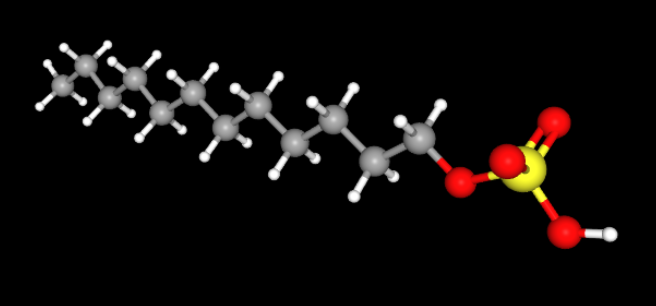
\includegraphics[width=0.7\textwidth]{archivos/SDS.PNG}
	\caption{Sodium dodecyl sulfate (SDS) molecule~\cite{SDS} (white=H, grey=C, red=O, yellow=S; sodium cation, $Na+$, not represented)}
	\label{refraction}
\end{figure}

Sodium dodecyl sulfate~\cite{SDS}, also known as Sodium Lauryl Sulfate (SLS) is an anionic surfactant naturally derived from coconut and/or palm kernel oil. SDS also has some microbicidal activity. Its molecular formula is $C_{12}H_{25}O_4S.Na$ and its molecular Weight, $288.38 \; \textrm{g/mol}$.

\begin{figure}[H]
	\centering
	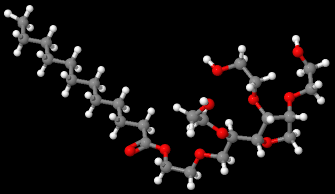
\includegraphics[width=0.7\textwidth]{archivos/Tween20.PNG}
	\caption{Simplified (missing PEG units) Polysorbate 20 (Tween® 20) molecule (white=H, grey=C, red=O)~\cite{Tween}(modified image)}
	\label{tween}
\end{figure}

Polysorbate 20 is a synthetic nonionic surfactant. The number 20 corresponds to the 20 repeat units of polyethylene glycol (PEG) in the polar head of the molecule. These units are distributed across 4 different chains, so in fact Polysorbate 20 consists of a range of chemical species.

Trace amounts of this substances lower the surface tension, helping the setup and improving the durability of the film. In the beginning we used SDS in low concentrations (always lower than its CMC, $8.2 \; \textrm{mM}$ at $25^\textrm{o} \textrm{C}$) in some films. Later, based on the paper of Kurtuldu et al.~\cite{Kurtuldu2011}, we used Tween 20, $0.03\%$ v~∕~v in some of our experiments.

\section{Staining}
\label{mm_staining}

In some experiments, if the initial thickness of the film was too high, and therefore, the evaporation time, very long, the algae would eventually stop moving before reaching the desired thickness, hampering the production of meaningful images/data.

This lack of motion can be due to either the death of the cells or the loss of their flagella. To know if it is one or the other, we decided to conduct a LIVE/DEAD Cell test. 

The test kit we will be using consists of calcein acetoxymethyl (\textit{calcein AM}) and ethidium homodimer-1 (\textit{EthD-1}). The former is a non-fluorescent compound that can be transported through the cellular membrane. Once inside the cell, the intracellular esterase activity removes the acetomethoxy group, so the molecule can no longer exit the cell and it exhibits a strong green fluorescence. The latter is a membrane-impermeable, high-affinity nucleic acid red stain that is weakly fluorescent until bound to DNA. When cells die, the plasma membranes break down, letting EthD-1 enter.

Noise levels out of the cells are weak since both dyes are almost non-fluorescent before interaction with the cells.

In conclusion, the test should show live cells stained with Calcein-AM (green) and dead cells with EthD-1 (red). Nonetheless, it should be noted that the test kit we will use is designed for mammalian cells (ThermoFisher Scientific LIVE/DEAD™ Viability/Cytotoxicity Kit, for mammalian cells: ref. L3224). \textit{Chlamydomonas reinhardtii} presents a cell wall which, although cellulose-deficient~\cite{Imam}, may interfere with the staining. Nonetheless, previous successful experiences with bacteria, that are also wrapped in a cell wall, encourage the realization of the experiment. 

The original protocol for mammalian cells is the following one:

\begin{itemize}
	\item Prepare $2 \; \mu \textrm{L}$ calcein and $4 \; \mu \textrm{L}$ Eth-D in 1mL EC media.
	\item Wash system with PBS
	\item Inject live/dead in the system, place in incubator for 30 minutes.
	\item Remove live/dead and wash with PBS. Wait for 5 minutes.
	\item Refresh PBS. Wait for 5 minutes.
	\item Image live/dead.
\end{itemize}

It is intended to discern which cells are dead or alive at the time when they are stained. We, on the contrary, would like to acquire a more \textit{dynamic} information: if cells that were alive at the beginning of the experiment are dying over it. This is why our protocol becomes:

\begin{itemize}
	\item Centrifugate ($600 \; \textrm{g}$, $6 \; \textrm{minutes}$) and replace the algae medium (TAP) 3 times.
	\item Get 0.2mL of the desired concentration by centrifugation. 
	\item Prepare $2 \; \mu \textrm{L}$ calcein and $4 \; \mu \textrm{L}$ Eth-D in $0.8 \; \textrm{mL}$ TAP media.
	\item Wash system with ethanol.
	\item Wash system with distilled water.
	\item Inject live/dead in the system.
	\item Image live/dead.
\end{itemize}

%https://www.thermofisher.com/order/catalog/product/L3224
